%\section{The prop $\M$}

\subsection{Operads and props} \label{s:operads and props}

Let $\S$ be the category whose objects are the natural numbers and whose set of morphisms between $m$ and $n$ is empty if $m \neq n$ and is otherwise the symmetric group $\S_n$.
A \textit{left $\S$-module} (resp. \textit{right} $\S$-\textit{module} or $\S$-\textit{bimodule}) is a covariant functor from $\S$ (resp. $\S^\op$ or $\S \times \S^\op$) to $\Ch$.
In this paper we prioritize left module structures over their right counterparts. As usual, taking inverses makes both perspectives equivalent.
We respectively denote by $\smod$ and $\sbimod$ the categories of left $\S$-modules and of $\S$-bimodules with morphisms given by natural transformations.

The collections of group homomorphism $\S_n \to \S_n \times \S_1$ for $n \geq 0$ induces a forgetful functor $U \colon \sbimod \to \smod$.
The similarly defined forgetful functor to right $\S$-modules will not be used.

Given an object $C$ in $\C$ define:
\begin{align*}
\End^C(r) &= \Hom(C, C^{\otimes r}),
&\End^C_C(r, s) &= \Hom(C^{\otimes r}, C^{\otimes s}),
\end{align*}
with their natural structures of $\S$-module and $\S$-bimodule respectively.
The forgetful functor $U$ sends $\End^C_C$ to $\End^C$.

We can define \textit{operads} and \textit{props} by enriching $\S$-modules and \mbox{$\S$-bimodules} with certain composition structures.
For a complete presentation of these concepts we refer to Definition 11 and 54 of \cite{Markl08}.
Intuitively, operads and props can be understood by abstracting the composition structure naturally present in the left $\S$-module $\End^C$, naturally an operad, and the $\S$-bimodule $\End^C_C$, naturally a prop.
We remark that the structure on a prop $\P$ restricts to an operad structure on $U(\P)$.

We can also think of operads and props as algebras over the monad associated to the free-forgetful adjunctions
\begin{equation*}
\begin{tikzcd}
\smod \arrow[r, bend left] & \arrow[l, bend left] \operads 
& \text{and} &
\sbimod \arrow[r, bend left] & \arrow[l, bend left] \props
\end{tikzcd}
\end{equation*}
which we now review, see \cite{Markl08} or \cite{Fresse2010props} for a more detailed presentation.

The \textit{free prop} $F(M)$ generated by an \mbox{$\S$-bimodule} $M$ is constructed using open directed graphs with no directed loops that are enriched with a labeling described next. We think of each directed edge as built from two compatibly directed half-edges. For each vertex $v$ of a directed graph $G$, we have the sets $in(v)$ and $out(v)$ of half-edges that are respectively incoming to and outgoing from $v$. Half-edges that do not belong to $in(v)$ or $out(v)$ for any $v$ are divided into the disjoint sets $in(G)$ and $out(G)$ of incoming and outgoing external half-edges. For any positive integer $n$ let $\overline{n} = \{1,\dots,n\}$ and set $\overline{0} = \emptyset$. For any finite set $S$, denote the cardinality of $S$ by $|S|$. The labeling is given by bijections  
\begin{equation*}
\overline{|in(G)|}\to in(G), \qquad
\overline{|out(G)|}\to out(G),
\end{equation*}
and
\begin{equation*}
\overline{|in(v)|}\to in(v), \qquad
\overline{|out(v)|}\to out(v),
\end{equation*}
for every vertex $v$.
We refer to the isomorphism classes of such labeled directed graphs with no directed loops as $(n,m)$\textit{-graphs} denoting the set of these by $\G(m,n)$.
We use graphs immersed in the plane to represent elements in $\G(m,n)$, please see Figure \ref{f:immersion}.
We consider the right action of $\S_n$ and the left action of $\S_m$ on a $(n,m)$-graph given respectively by permuting the labels of $in(G)$ and $out(G)$. This action defines the $\S$-bimodule structure on the free prop
\begin{equation} \label{e:free prop}
F(M)(m,n) \ = \bigoplus_{\Gamma \in \G(m,n)} \bigotimes_{v \in Vert(\Gamma)} out(v) \otimes_{\S_q} M(p, q) \otimes_{\S_p} in(v),
\end{equation}
where we simplified the notation writing $p$ and $q$ for $\overline{|in(v)|}$ and $\overline{|out(v)|}$ respectively. The composition structure is defined by (relabeled) grafting and disjoint union.
The free operad is constructed similarly only using $(1,m)$-graphs.

Let us now focus on the category $\Ch$.
Let $C$ be a chain complex, $\O$ an operad, and $\P$ a prop.
An $\O$-\textit{coalgebra} (resp. $\O$-\textit{algebra} or $\P$-\textit{bialgebra}) structure on $C$ is a structure preserving morphism $\O \to \End^C$ (resp. $\P \to \End_C^C$).

An $\S$-module $M$ is said to be $E_\infty$ if for each $r$ the chain complex $M(r)$ is an algebraic model for the universal bundle $E\S_r$, i.e., it is free as an $\S_r$-module and its homology is that of a point.
An operad is said to be $E_\infty$ if its underlying $\S$-modules is $E_\infty$.
A prop $\P$ is said to be $E_\infty$ if $U(\P)$ is an $E_\infty$ operad.

\begin{figure}
	\begin{tikzpicture}[scale=.6]
\draw (1,3.7) to (1,3); 

\draw (1,3) to [out=205, in=90] (0,0);

\draw [shorten >= 0cm] (.6,2.73) to [out=-100, in=90] (2,0);

\draw [shorten >= .15cm] (1,3) to [out=-25, in=30, distance=1.1cm] (1,1.5);
\draw [shorten <= .1cm] (1,1.5) to [out=210, in=20] (0,1);

\node at (1,3.9){};
\node at (0,-.32){};
\node at (2,-.32){};

\node at (3,1.5){$\sim$\ \ \ };
\end{tikzpicture}
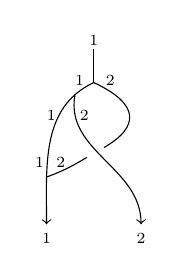
\begin{tikzpicture}[scale=.6]
\draw (1,3.7) to (1,3); 

\draw [->](1,3) to [out=205, in=90] (0,0);

\draw [shorten >= 0cm,->] (.6,2.73) to [out=-100, in=90] (2,0);

\draw [shorten >= .15cm] (1,3) to [out=-25, in=30, distance=1.1cm] (1,1.5);
\draw [shorten <= .1cm] (1,1.5) to [out=210, in=20] (0,1);


\def\x{.8}

\node[scale=\x] at (1,3.9){$\scriptstyle 1$};

\node[scale=\x] at (.7,3.05){$\scriptstyle 1$};
\node[scale=\x] at (1.35,3.05){$\scriptstyle 2$};

\node[scale=\x] at (.1,2.3){$\scriptstyle 1$};
\node[scale=\x] at (.8,2.3){$\scriptstyle 2$};

\node[scale=\x] at (-.15,1.3){$\scriptstyle 1$};
\node[scale=\x] at (.3,1.3){$\scriptstyle 2$};

\node[scale=\x] at (0,-.3){$\scriptstyle 1$};
\node[scale=\x] at (2,-.3){$\scriptstyle 2$};
\end{tikzpicture}
	\caption{Immersed graphs represent labeled directed graphs with the direction implicitly given from top to bottom and the labeling from left to right.}
	\label{f:immersion}
\end{figure}

\subsection{The prop $\M$}\label{propM}

Let us consider the free prop $F(N)$ generated by the $\S$-bimodule $N$ whose only non-zero chain complexes are concentrated in degree $0$ and are give by
\begin{equation*}
N(1, 0) = R\{\varepsilon\}, \qquad
N(1, 2) = R[\S_2]\{\Delta\}.
\end{equation*}
Define $\As$ as the quotient of $F(N)$ by the prop ideal generated by the relations
\begin{equation*}
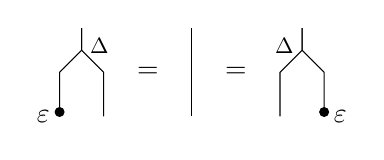
\begin{tikzpicture}[scale=.28]
\draw (-4,0)--(-4,2)--(-5,3)--(-5,4);
\draw (-6,0)--(-6,2)--(-5,3)--(-5,4);
\node [scale=.8] at (-4.2,3.2) {$\Delta$};
\draw [fill] (-6,.2) circle [radius=.2];
\node [left] at (-6,0) {$\varepsilon$};

\node at (-2,2) {=};
\draw (0,0)--(0,4);
\node at (2,2) {=};

\draw (4,0)--(4,2)--(5,3)--(5,4);
\draw (6,0)--(6,2)--(5,3)--(5,4);
\node [scale=.8] at (4.2,3.2) {$\Delta$};
\draw [fill] (6,.2) circle [radius=.2];
\node [right] at (6,0) {$\varepsilon$};
\end{tikzpicture}
\qquad \qquad
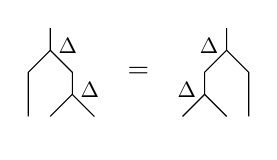
\begin{tikzpicture}[scale=.28]
\node at (0,2){=};
\node at (0,0) {\phantom{$\varepsilon$}};

\draw (2,0)--(3,1)--(3,2)--(4,3)--(4,4);
\draw (4,0)--(3,1);
\draw (4,3)--(5,2)--(5,0);
\node [scale=.8] at (3.2,3.2) {$\Delta$};
\node [scale=.8] at (2.2,1.2) {$\Delta$};

\draw (-2,0)--(-3,1)--(-3,2)--(-4,3)--(-4,4);
\draw (-4,0)--(-3,1);
\draw (-4,3)--(-5,2)--(-5,0);
\node [scale=.8] at (-3.2,3.2) {$\Delta$};
\node [scale=.8] at (-2.2,1.2) {$\Delta$};
\end{tikzpicture}
\end{equation*}
We remark that the category $\coAlg_{U(\As)}$ is equivalent to $\coAlg$.

Let $W^{(1)}$ be the chain complex of free $R[\S_2]$-modules
\begin{equation*}
\begin{tikzcd}
R[\S_2]\{\nu\} &[0pt] \arrow[l, "1-T"'] R[\S_2]\{\mu\},
\end{tikzcd} 
\end{equation*}
which is isomorphic to the cellular chains on the standard $\S_2$-equivariant $CW$-structure on the circle
\begin{equation*}
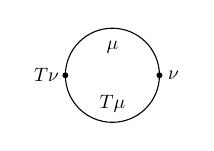
\begin{tikzpicture}[scale=.85]
\draw (0,0) circle (20pt);
\node[scale=.7] at (0,12pt){$\mu$};
\node[scale=.7] at (0,-12pt){$T \mu$};
\node[scale=.7] at (-28pt,0){$T \nu$};
\node[scale=.7] at (26pt,0){$\nu$};
\draw [fill] (-20pt,0) circle [radius=1pt];
\draw [fill] (20pt,0) circle [radius=1pt];
\end{tikzpicture}
\end{equation*}
and let $W^{(0)}$ be the subcomplex generated by $\nu$. We think of $W^{(1)}$ as an $\S_2$-equivariant 1-cell with boundary $W^{(0)}$.

We regard these complexes as $\S$-bimodules concentrated in biarity $(2,1)$, and let $\varphi \colon W^{(0)} \to \As$ be define by sending $T \nu$ and $\nu$ respectively to
\begin{equation*}
\begin{tikzpicture}[scale=.2]
\draw (-4,0)--(-4,4);
\draw (-6,0)--(-6,4);
\draw [fill] (-6,.2) circle [radius=.2];
\node [left] at (-6,0) {$\varepsilon$};

\node at (0,.4) {and};

\draw (4,0)--(4,4);
\draw (6,0)--(6,4);
\draw [fill] (6,.2) circle [radius=.2];
\node [right] at (6,0) {$\varepsilon$.};
\end{tikzpicture}
\end{equation*}
Consider the push-out
\begin{equation*}
\begin{tikzcd}
F(W^{(0)}) \arrow[r, "F(\varphi)"] \arrow[d] & \As \arrow[d, dashed] \\
F(W^{(1)}) \arrow[r, dashed] & \mu \vee_\varphi \As
\end{tikzcd}
\end{equation*}
in the category of props. We think of $\mu \vee_\varphi \As$ as the prop obtained by attaching a $1$-cell in biarity $(2,1)$ to $\As$.

Define $\M$ as the quotient of $\mu \vee_\varphi \As$ by the ideal generated by
\begin{equation*}
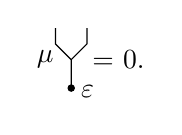
\begin{tikzpicture}[scale=.2]
\draw (5,4)--(5,3)--(6,2)--(6,0);
\draw (7,4)--(7,3)--(6,2);
\node [left] at (5.5,2) {$\mu$};
\draw [fill] (6,.2) circle [radius=.2];
\node [right] at (6,0) {$\varepsilon$};

\node at (9,2) {= 0.};
\end{tikzpicture}
\end{equation*}

We can give a more explicit description of $\M$ using the description of the free prop in terms of $(m,n)$-graphs.
Consider the following elements in $\M$
\begin{equation*}
\counit \in \mathcal M(1,0)_0, \hspace*{.6cm} \coproduct \in \mathcal M(1,2)_0, \hspace*{.6cm} \product \in \mathcal M(2,1)_1,
\end{equation*}
where the decorations by $\varepsilon$, $\Delta$, and $\mu$ are omitted.
Any element in $\M(m,n)$ can be written as a linear combination of the $(m,n)$-graphs generated by these three by grafting, disjoint union and relabeling, modulo the ideals generated by the relations
\begin{equation*}
\qquad \leftcounitality \, , \qquad \rightcounitality \, , \qquad \coassociativity \, , \qquad \productcounit \, .
\end{equation*}
Its chain complex structure is determined using \eqref{e:free prop} by 
\begin{equation*}
\partial\ \counit = 0, \hspace*{.6cm} \partial \ \coproduct = 0, \hspace*{.6cm} \partial \ \product = \ \boundary \, .
\end{equation*}

The following result was shown in \cite{Medina20prop1}.

\begin{proposition}
	The prop $\M$ is an $E_\infty$-prop.
\end{proposition}

Since $\As$ includes into $\M$, there is a functor between the corresponding categories of coalgebras $\coAlg_{U(\M)} \to \coAlg_{U(\As)} = \coAlg$.
